%
% auth: Mattijs Korpershoek
% mail: <mattijs.korpershoek@gmail.com>
%

% {{{1 intro

% {{{1 Opensourcing
\section{Open-sourcing the Parameter-framework}

\currentSectionToc

\subsection{Documentation}
\begin{frame}
    \frametitle{Newcomer documentation}
    \centering
    \begin{block}{Is the component ready for open-sourcing?}
        \begin{itemize}
            \item Code review and study
            \item Documentation for external contributors
            \item More than 450 lines of documentation
        \end{itemize}
    \end{block}
\end{frame}

\begin{frame}
    \frametitle{Newcomer documentation illustration}
    \centering
    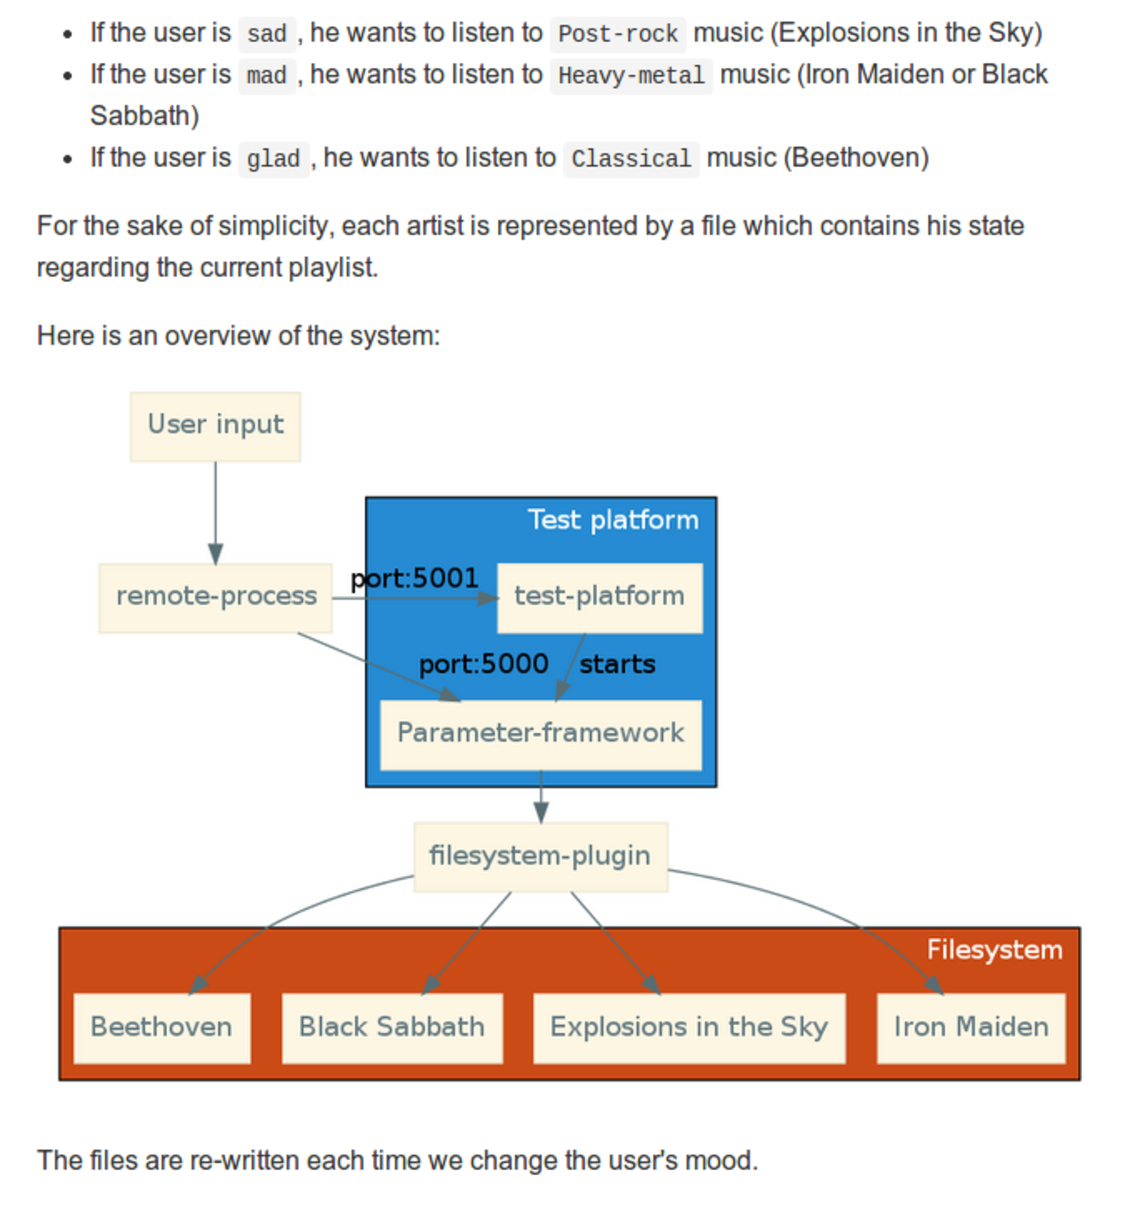
\includegraphics[height=0.85\textheight]{../../report/src/img/tutos.pdf}
\end{frame}

\subsection{Open-sourcing topics}
\begin{frame}
    \frametitle{Open-sourcing problems and solutions}
    \begin{block}{Confidential information should not be exposed}
        \begin{itemize}
            \item Refactor code to move parts to separate projects
        \end{itemize}
    \end{block}
    \begin{block}{External contributions should not break internal functionalities}
        \begin{itemize}
            \item TODO
        \end{itemize}
    \end{block}
    \begin{block}{GitHub and internal source tree should contain same code}
        \begin{itemize}
            \item Ensure common
        \end{itemize}
    \end{block}
\end{frame}

\begin{frame}
    \frametitle{GitHub top contributors}
    \centering
    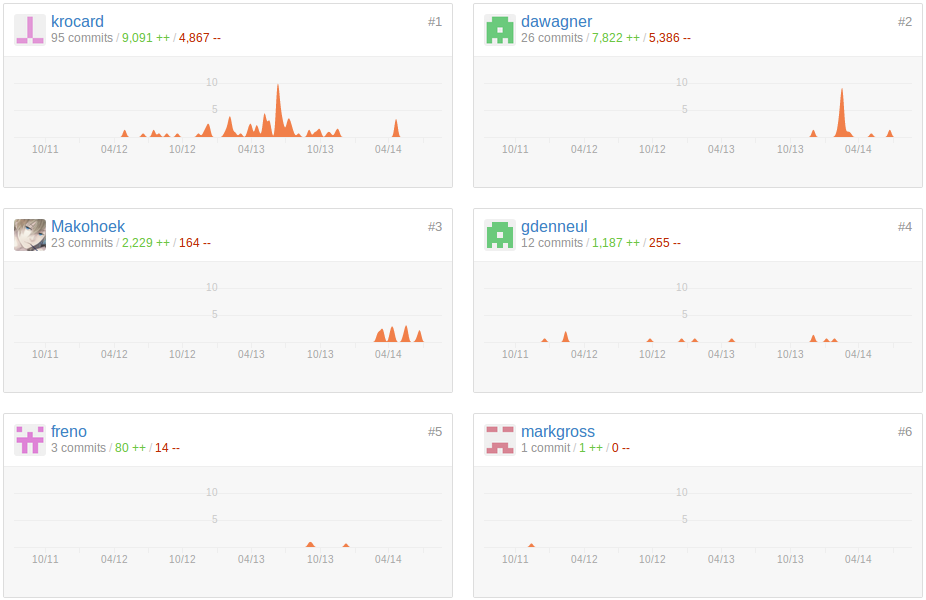
\includegraphics[width=\textwidth]{../../report/src/img/statsGitHub.png}
\end{frame}

\subsection{Outcome}
\begin{FrameWithSubSection}
    \frametitle{Projects which are open-source}
    \begin{minipage}{0.6\textwidth}
        \begin{itemize}
            \item \href{https://01.org/}{\color{blue}Intel Open Source Technology Center}
            \item \href{https://github.com/orgs/01org/teams/01-org-parameter-framework-owners}{\color{blue}GitHub organisation}
        \end{itemize}
    \end{minipage}
    \begin{minipage}{0.35\textwidth}
        \flushright
        
\includegraphics[width=\textwidth]{./img/01orglogo.png} \\
        
\includegraphics[height=1cm]{./img/githubLogo.png}
    \end{minipage}
    \begin{block}{Projects on GitHub}
        \begin{itemize}
            \item Parameter-framework \href{https://github.com/01org/parameter-framework}{\color{blue}core}
            \item Parameter-framework \href{https://github.com/01org/parameter-framework-plugins-alsa}{\color{blue}ALSA plugin}
            \item Parameter-framework \href{https://github.com/01org/parameter-framework-plugins-filesystem}{\color{blue}filesystem plugin}
            \item Parameter-framework \href{https://github.com/01org/parameter-framework/wiki}{\color{blue}wiki}
            \item Parameter-framework \href{https://github.com/01org/parameter-framework-samples}{\color{blue}sample files}
        \end{itemize}
    \end{block}
\end{FrameWithSubSection}

